\subsection{SFT with Variable-Length CoT Data}
\label{sec:longshortdata}


\textbf{\textit{Fine-tuning LLMs with variable-length CoT data}} is an effective way to improve the efficiency of reasoning. As shown in Figure~\ref{fig:sft}, this series of works typically involves: (1) Constructing variable-length CoT reasoning datasets via various methods, and (2) Applying SFT with collected data on reasoning models to enable LLMs to learn compact reasoning chains that encapsulate effective knowledge. Note that this method is not limited to RL-trained reasoning models; it can also directly enhance reasoning models by injecting efficient reasoning capabilities, similar to those used in distilled reasoning models.(e.g., DeepSeek-R1-Distill-Qwen~\cite{guo2025deepseek}).

\insightbox{The key question is: How to collect variable-length CoT reasoning data, especially for short CoT data?}

\begin{figure}[h]
    \centering
    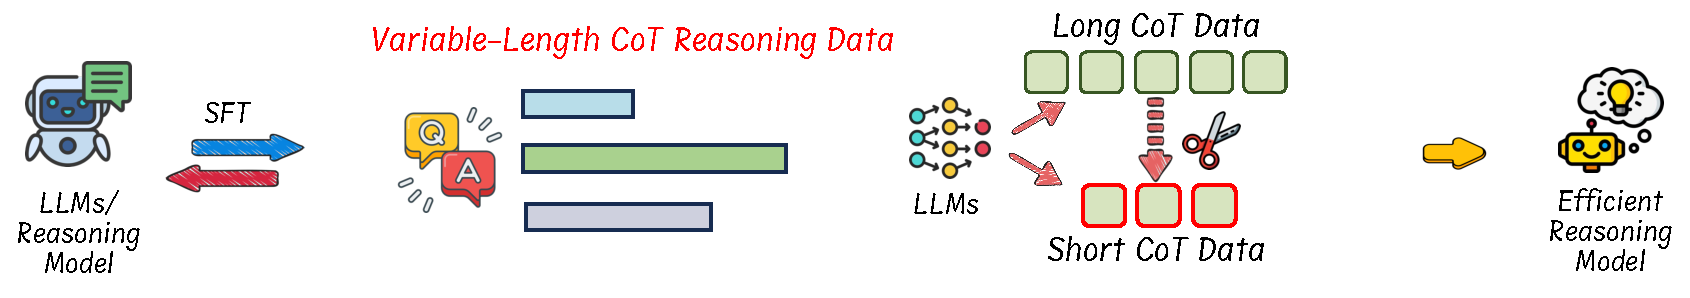
\includegraphics[width=\linewidth]{figs/sft.pdf}
    % \vspace{1mm}
    \caption{Illustration of methods for utilizing SFT with variable-length CoT reasoning datasets.}
    \label{fig:sft}
\end{figure}

\begin{table}[ht]
\centering
\small
\caption{Comparison of various approaches that utilize SFT with variable-length CoT reasoning datasets.}
\label{tab:variable-length}
\resizebox{\textwidth}{!}{
\begin{tabular}{l|cccccccccc}
\toprule
\textbf{Method} & \textbf{Source Data} & \textbf{Reasoning Pruning} & \textbf{SFT} & \textbf{LLMs} \\
\midrule\midrule
Self-Training~\cite{munkhbat2025self} & \makecell[c]{GSM8K \\ MATH} & \makecell[c]{Sampling $N$ \\ reasoning then select \\ the shortest one}  & Standard & \makecell[c]{Llama-3.2-\{1B,3B\} \\ Llama-3.1-8B} \\ % \makecell[c]{Llama-3.2-\{1B,3B\} \\ Gemma2-2B \\ Qwen2.5-3B \\ Qwen2.5-Math-1.5B \\ DeepSeekMath-7B}
\midrule
TokenSkip~\cite{xia2025tokenskip} & \makecell[c]{GSM8K \\ MATH} & \makecell[c]{Skip tokens according to \\ semantic importance} & Standard & \makecell[c]{LLaMA-3.1-8B-Instruct \\ Qwen2.5-Instruct} \\
\midrule
C3oT~\cite{kang2024c3ot} & \makecell[c]{GSM8K \\ MathQA \\ ECQA \\ StrategyQA} & \makecell[c]{GPT-4 as compressor \\ to make concise \\ reasoning} & Standard & Llama-2-chat-\{7B,13B\} \\
\midrule
Distilling2-1~\cite{yu2024distilling} & OASST2 & Removing reasoning & Standard & Llama-2-70B-chat \\
\midrule
Token-Budget~\cite{han2024token} & \makecell[c]{GSM8K \\ GSM8K-Z \\ MathBench} & \makecell[c]{Persuing an optimal \\ token budget for LLMs \\ to complete the reasoning} & Standard & Llama-3.1-8B-Instruct \\
\midrule
CoT-Valve~\cite{ma2025cot} & \makecell[c]{GSM8K \\ PRM800k} & \makecell[c]{Merging parameters \\ of non-reasoning and \\ long reasoning LLMs} & Progressive & \makecell[c]{QwQ-32B-Preview \\ DeepSeek-R1-Distill-Llama-8B \\ LLaMA-3.1-8B \\ LLaMA-3.2-1B \\ Qwen32B-Instruct} \\
\midrule
LearnSkip~\cite{liu2024can} & \makecell[c]{Analog of Algebra \\ Multi-digit Addition \\ Directional Reasoning} & \makecell[c]{Stage 1: Manually skipping \\ Stage 2: Prompting LLMs \\ for shorter reasoning} & \makecell[c]{Standard \& \\ Progressive} & \makecell[c]{Llama-2-7B \\ Phi-3-mini~(3.8B)} \\
\bottomrule
\end{tabular}
}
\end{table}

\subsubsection{Constructing Variable-Length CoT Reasoning Datasets}

%
Variable-length CoT reasoning datasets refer to datasets of long/short reasoning steps that could guide LLMs to achieve correct answers.
%
Existing works typically gather long CoT data by prompting pre-trained reasoning models with questions. Based on the long CoT data, the key challenge is: \textit{How to collect short CoT data?} Overall, variable-length CoT reasoning datasets can be created via either post-reasoning or during-reasoning. We list some detailed approaches in Table~\ref{tab:variable-length}.

\paragraph{\textbf{Post-reasoning CoT Compression.}}
This approach collects short CoT data by reducing redundant reasoning steps after full-length reasoning, either by heuristic criterion or LLMs, as proposed in \cite{yu2024distilling},~\cite{kang2024c3ot}, and~\cite{xia2025tokenskip}.  
Specifically, \cite{yu2024distilling} uses reasoning-capable LLMs to generate the reasoning and answers. After generating full-length CoT data, they discard the reasoning process, only using the questions and answers to distill system-1 LLMs.
Another work C3oT improves the reasoning efficiency by compressing the reasoning process~\cite{kang2024c3ot}. The long CoT reasoning steps were generated by explicitly prompting LLMs. Then, it employs GPT-4 as a compressor to reduce the length of the reasoning process while ensuring the compressed reasoning retains all key information and removes redundant words. In addition, TokenSkip reduce the reasoning steps driven by interpretation~\cite{xia2025tokenskip}.
It estimates the semantic importance of each reasoning part to the final answer and reduces the reasoning tokens.
The important parts preserve the key reasoning steps that could improve the accuracy of the final answer.
The advantage of post-reasoning CoT compression is that it can achieve a higher reduction rate of the reasoning steps, which advances more efficient reasoning.

\paragraph{\textbf{Obtaining Compressed CoT Data during Reasoning.}}
This approach collects short CoT data by prompting LLMs to generate short reasoning steps during inference and reasoning, as proposed in \cite{liu2024can}, \cite{munkhbat2025self},~\cite{han2024token}, and~\cite{ma2025cot}.
Specifically, \cite{liu2024can} proposes a human-like step-skipping method for generating shorter reasoning steps. In the first stage, based on the original training datasets, they manually create solutions by skipping steps, either guided by human expertise or by randomly merging or removing steps. Further, these concise data are labeled with prompts such as “Solve it in $n$ steps.”. After SFT, the model is able to generate shorter reasoning paths. In the second stage, they prompt this model to solve problems by intrinsically skipping or compressing steps during reasoning.
The generated concise reasoning steps with questions and answers are collected as datasets, which are then used in SFT to make LLMs solve problems with fewer steps.
Moreover, Token-Budget~\cite{han2024token} has an important insight: an optimal token budget helps LLMs actively follow the token constraint to complete the reasoning process.
Motivated by this insight, it proposes a binary search-based method to achieve the optimal token budgets, and follow these budgets to generate short reasoning steps. 
In addition, \cite{munkhbat2025self} proposes a sampling-based method to improve reasoning efficiency.
Specifically, it examines the distribution of reasoning lengths and finds that shorter solutions appear more frequently than the typical reasoning length.
Driven by this finding, it proposes a Best-of-N~(BoN) Sampling at test time, which generates $N$ paths of reasoning and selects the shortest one.
These short reasoning paths are collected as the dataset.
Finally, CoT-Valve~\cite{ma2025cot} controls the reasoning length by mix-up the parameters of long reasoning and non-reasoning LLMs for generating variable-length reasoning steps.
The advantage of CoT compression during reasoning is that the naturally generated reasoning steps align with the intrinsic knowledge of LLMs, which advances more effective learning of LLMs.

\subsubsection{Fine-Tuning Approaches}

After collecting variable-length CoT data, existing works fine-tune LLMs to achieve efficient reasoning in several ways, which include standard fine-tuning (e.g., parameter-efficient fine-tuning such as LoRA~\cite{hu2022lora} or full fine-tuning) and progressive fine-tuning.

\paragraph{\textbf{Standard Fine-tuning.}}
Most of the work adopts standard methods to fine-tune LLMs~\cite{liu2024can, munkhbat2025self, yu2024distilling, kang2024c3ot, xia2025tokenskip, han2024token}. 
Specifically, these approaches adopt LoRA~\cite{hu2022lora} or full fine-tuning~\cite{kang2024c3ot} to minimize the perplexity loss function or DPO loss function~\cite{han2024token} on the reasoning-efficient datasets.
The LoRA enables LLMs to adapt to short reasoning steps with less than $1\%$ of the parameters tuned.
In addition, \cite{liu2024can} observed the growing reasoning efficiency can generalize to out-of-domains beyond the collected datasets.

\paragraph{\textbf{Progressive Fine-tuning.}}
Progressive fine-tuning aims to smoothly reduce the reasoning steps during fine-tuning~\cite{ma2025cot, liu2024can}.
One way is to progressively reduce the reasoning steps of data during fine-tuning LLMs, as employed in \cite{liu2024can}.
Another effective way is to progressively adjust the generation of reasoning steps, as proposed by CoT-Valve~\cite{ma2025cot}. 
Specifically, it first learns LoRA adaptor $\Delta \theta_{\text{N}}$ and $\theta_{\text{L}}$, where LLMs with $\Delta \theta_{\text{N}}$ have no reasoning steps, and that with $\Delta \theta_{\text{L}}$ have long reasoning.
Then, it mix-up $\Delta \theta_{\text{N}}$ and $\Delta \theta_{\text{long}}$ by  
$\alpha \Delta \theta_{\text{N}} + (1-\alpha) \Delta \theta_{\text{L}}$ to generate a dataset reasoning with variable length.
Here $0 < \alpha < 1$ controls the parameter to shift from $\Delta \theta_{\text{N}}$ to $\Delta \theta_{\text{L}}$, controlling the reasoning length generated by LLMs.
Finally, it fine-tunes LLMs on the generated data while progressively reducing $\alpha$ from 1 to 0.
In this way, reasoning efficiency is progressively improved during fine-tuning.

\paragraph{Model Merging.} Beyond fine-tuning reasoning models using the above CoT data, several works have explored model merging to improve reasoning efficiency in LLMs. Kimi k1.5~\cite{team2025kimi} investigates merging strategies~\cite{yang2024modelmergingllmsmllms} that transform models producing lengthy CoT traces into ones that generate shorter, more concise reasoning outputs. Unlocking~\cite{wu2025unlockingefficientlongtoshortllm} conducts an empirical study on model merging for efficient reasoning with various methods, including task-vector-based, SVD-based, and activation-informed merging. 